\documentclass[11pt]{article} \usepackage[margin=1in]{geometry}
\usepackage[T1]{fontenc} \usepackage[utf8]{inputenc} \usepackage{lmodern}
\usepackage{array} \usepackage{booktabs} \usepackage{enumitem}
\usepackage{setspace} \usepackage{titlesec}
\usepackage{tikz}
\usepackage{url}
\usetikzlibrary{arrows.meta,positioning}

% Misc
\newcommand{\bert}[1]{\textcolor{cyan}{[BJD: #1]}}
\newcommand{\bertmargin}[1]{\marginpar{\fontsize{6pt}{6pt}\selectfont\raggedright\textcolor{cyan}{BJD: #1}}}

\newcommand{\wyatt}[1]{\textcolor{green}{[WJH: #1]}}
\newcommand{\wyattmargin}[1]{\marginpar{\fontsize{6pt}{6pt}\selectfont\raggedright\textcolor{green}{WJH: #1}}}

\setlength{\parindent}{0pt} \setlength{\parskip}{0.35em}
\setlist[itemize]{leftmargin=1.5em, itemsep=0.2em, topsep=0.2em}
\titleformat{\section}{\normalfont\bfseries}{\thesection.}{0.5em}{}
\titleformat{\subsection}{\normalfont\bfseries}{\thesubsection.}{0.5em}{}

% Title-page fields
\newcommand{\ProjectTitle}{GENESIS-AGENT: A Generative Engine for Novel,
Explainable, Secure, and Integrated Simulation with Agentic Artificial Intelligence} \newcommand{\LeadInstitution}{Sandia National Laboratories}
\newcommand{\StreetAddress}{TBD} \newcommand{\PostalAddress}{TBD}
\newcommand{\LeadPI}{TBD} \newcommand{\LeadPIContact}{TBD}
\newcommand{\AdminPOC}{TBD} \newcommand{\AdminPOCContact}{TBD}
\newcommand{\RFANumber}{DE-FOA-0003612} \newcommand{\PrimaryChallenge}{19 -- AI
for Scientific Reasoning} \newcommand{\PrimaryFocusArea}{A/B/C -- Trustworthy
Mathematical and Symbolic Reasoning; Hypothesis Generation from Multi-Modal
Data; Composable and Modular Foundation Models}
\usepackage{comment}
\begin{document}

\pagenumbering{gobble} \begin{titlepage} \thispagestyle{empty} \begin{center}
{\Large \textbf{\ProjectTitle}\par} \end{center}

\vspace{1em} \textbf{Lead Applicant/Institution:} \LeadInstitution

\textbf{Street Address:} \StreetAddress

\textbf{Postal Address:} \PostalAddress

\textbf{Lead PI name, telephone number, email:} \LeadPI; \LeadPIContact

\textbf{Administrative Point of Contact name, telephone number, email:}
\AdminPOC; \AdminPOCContact

\textbf{RFA Number:} \RFANumber

\textbf{Primary challenge and focus area:} \PrimaryChallenge{} $|$
\PrimaryFocusArea

\vspace{1em} \textbf{Senior/Key Personnel for Lead Institution and All Partner
Institutions}

\begin{tabular}{p{0.35\textwidth} p{0.6\textwidth}} \toprule \textbf{Institution
Name} & \textbf{Senior/Key Personnel including the Director} \\ \midrule
\LeadInstitution{} (Lead) & TBD \\ Partner Institution 1 & TBD \\ Partner
Institution 2 & TBD \\ \bottomrule \end{tabular}

\vspace{1em} \textbf{Summary budget information for lead institution and all
partner institutions}

\begin{tabular}{p{0.65\textwidth} p{0.25\textwidth}} \toprule
\textbf{Institution} & \textbf{Year 1 Budget \$} \\ \midrule \LeadInstitution{}
(Lead) & TBD \\ Partner Institution 1 & TBD \\ Partner Institution 2 & TBD \\
\textbf{Total} & TBD \\ \bottomrule \end{tabular} \end{titlepage}

\clearpage \pagenumbering{arabic}



\section{Background/Introduction} 
Agentic artificial intelligence (AI) is poised to transform computational
science within DOE.  Traditionally, progress within computational
science has depended on the ability to generate a hypothesis from a myriad of
sources, translate this hypothesis to a computational study, analyze the
resulting data, and refine the next step.  In practice, this process requires
scientists and engineers to connect
scientific intent to outer-loop analyses, construct computational experiments,
execute large-scale simulation codes, analyze the results, and draw conclusions
or refine the experiment and repeat.  In many cases, the dominant bottleneck is
in this process not the cost of the computations, but the human effort required to generate,
execute, validate, and refine the study.

Recent advances in agentic AI are beginning to shift this paradigm. Commercial
systems such as Claude, Codex, and Cursor --- paired with frontier large language
models (LLMs) --- enable users to orchestrate complex workflows, autonomously
analyze results, and respond to sophisticated scientific queries. While these
capabilities have primarily emerged within coding environments, the underlying
LLMs and agentic technologies show strong promise for more ambitious scientific
workflows and underpin emerging concepts such as the ``AI Scientist''~\cite{lu2024aiscientistfullyautomated} and automated modeling and simulation in, for example, computational fluid dynamics~\cite{PaRaWa25,yue2026foamagentautomatedintelligentcfd,chen2024metaopenfoamllmbasedmultiagentframework,FENG2026100620} and finite element analysis~\cite{qi2025feagptendtoendagenticaifinite}. These developments point to a
transformative opportunity for the DOE enterprise.

Realizing this vision within DOE, however, requires significant advances.
Existing agentic systems have demonstrated success in constrained environments
with narrowly defined objectives, but scientific reasoning within DOE environments is inherently more diverse, often requiring cross-domain expertise and specialized experience. For example, workflows within DOE have multiple entry points, involve a myriad of analysis tools and a
broad range of simulation codes, each with distinct input formats, execution
requirements, and post-processing pipelines. Effective use of these tools also
requires detailed knowledge of HPC systems, data management, and
laboratory-specific operating constraints. Compounding this challenge, many DOE
codes are proprietary and absent from standard LLM training data. Enabling
agentic workflows in this setting therefore requires effective methods to synthesize
domain knowledge, software interfaces, and execution environments into
structured representations that AI systems can reliably use.
At the same time, scientific applications within DOE are often
high-consequence, where incorrect conclusions can lead to significant
downstream impacts. While agentic AI systems are powerful, they are not
infallible, and there remains a substantial trust gap between what these
systems can do and what users are willing to rely on. For these systems to be
useful for DOE analysis, they must be coupled to rigorous verification and validation 
and be designed to include human-in-the-loop oversight. Lastly, these technical challenges are further amplified by the security and operational
constraints of the DOE environment. Agentic AI systems within DOE must operate
under substantially stricter requirements than those in commercial or academic
settings, including constraints on data movement, the need for on-premises LLM deployments, and careful management of interactions between
agents and external tools. In particular, reliance on off-premises frontier
models and commercial software introduces risks related to data exposure and
reduced visibility and control over data and execution pathways. Ensuring
secure operation therefore requires robust sandboxing, fine-grained access
control, and verifiable policies governing tool use and system interactions.

\section{Project Objectives}
The objective of this project is to deliver \textbf{GENESIS-AGENT}: a
\textbf{G}enerative \textbf{E}ngine for \textbf{N}ovel, \textbf{E}xplainable,
\textbf{S}ecure, and \textbf{I}ntegrated \textbf{S}imulation with Agentic
AI, designed for deployment within the DOE ecosystem. Our long-term vision
(Phase II) is to develop an AI system capable of operating at the level of a
postdoctoral researcher: synthesizing scientific knowledge, formulating and
refining hypotheses, orchestrating computational experiments, and iteratively
improving conclusions under human supervision. A central premise is that
DOE-relevant agentic AI must be explicitly designed as a
\textit{human-in-the-loop} capability. While the agent may complete end-to-end
analyses, GENESIS-AGENT is structured so that human users remain directly
involved in reviewing plans, validating results, and refining
conclusions. %We view this as a core requirement for trustworthy AI in
%high-consequence computational science.
In Phase I, we will develop a minimal working framework that establishes the
foundations for this vision and demonstrates an initial AI advantage. We will
focus on end-to-end, agent-driven, human-in-the-loop workflows for a subset of
DOE tools, with emphasis on outer-loop problems such as inverse problems and
uncertainty quantification. Demonstrations will include candidate Sandia
software (e.g., Dakota for outer-loop analysis, SIERRA for computational
physics) and open-source tools (e.g., OpenFOAM). The goal is to reduce the
human effort required to formulate, validate, execute, and refine computational
studies while preserving expert oversight. Rather than manually constructing
studies and managing execution, users will leverage reusable agentic
infrastructure that accelerates workflow setup and iteration.

Realizing these objectives requires addressing several open research questions.
First, it remains unclear how agentic systems can scale reliably across the
diverse ecosystem of DOE tools, codes, and execution environments without
becoming too brittle or too narrowly tailored to a single workflow. Second, we
must determine what structured representations are needed for different parts of
the workflow so that agents can effectively reason over them. Finally,
verification remains an open challenge: we must develop methods to assess
whether agent-produced plans, inputs, and workflow decisions are correct,
reproducible, and trustworthy before they are used in high-consequence
computational studies.

%These objectives align directly with the chosen focus topic, \textit{AI for
%Scientific Reasoning}. GENESIS-AGENT is not limited to summarization or
%autocomplete; it is designed to reason across natural-language objectives,
%structured workflow specifications, scientific software interfaces, execution
%logs, and simulation outputs. By integrating model reasoning with formal
%workflow representations, retrieval, and controlled tool use, the project
%targets trustworthy mathematical and symbolic reasoning, multi-modal scientific
%context, and composable AI system design.


\section{Proposed Research and Methods}
%In Phase I, we propose to design and demonstrate a minimum working version of
%GENESIS-AGENT.
Our central hypothesis is that an AI advantage for scientific reasoning within DOE will not emerge from increasingly capable monolithic agents, but rather from role-specialized, multi-agent systems that integrate human-in-the-loop refinement.
%with structured representations of scientific workflows, multi-modal and retrieval-grounded reasoning, standardized tool interfaces, and iterative self-correction. 
To this end, we propose GENESIS-AGENT as a multi-agent framework for scientific reasoning in which task-specific agents rely on structured workflow representations to orchestrate and execute complex workflows. We will augment GENESIS-AGENT with retrieval-augmented generation (RAG)~\cite{lewis2021retrievalaugmentedgenerationknowledgeintensivenlp} pipelines to enable the synthesis of multimodal and proprietary information, and develop Model Context Protocol (MCP) servers to provide standardized access to tooling and enable plug-and-play coordination with different agentic technologies. 
These tools will be implemented in a closed loop fashion, enabling GENESIS-Agent to parse logs, identify errors, and feed this context into a correction loop. 




Our key innovations are: (i) structured workflow representations that enable agents to reason over complex outer-loop analyses; (ii) validation mechanisms to ensure correctness and reliability of agent-generated workflows; and (iii) a scalable, heterogeneous framework that supports interoperable and interchangeable agentic tools across diverse simulation ecosystems. To the best of our knowledge, the proposed work will comprise the first agentic technology designed to reason across multiple physics codebases and analysis drivers. 
This effort will build directly on co-Pi Dr. Pan's experience developing
Foam-Agent~\cite{yue2026foamagentautomatedintelligentcfd}, which is an agentic framework for translating natural-language requests into
executable OpenFOAM workflows. Foam-Aagent provides a concrete starting point
for several of the ideas proposed here, including retrieval over technical
documentation, code execution, and workflow verification and revision. 
\begin{comment}
\begin{figure}[t]
\centering
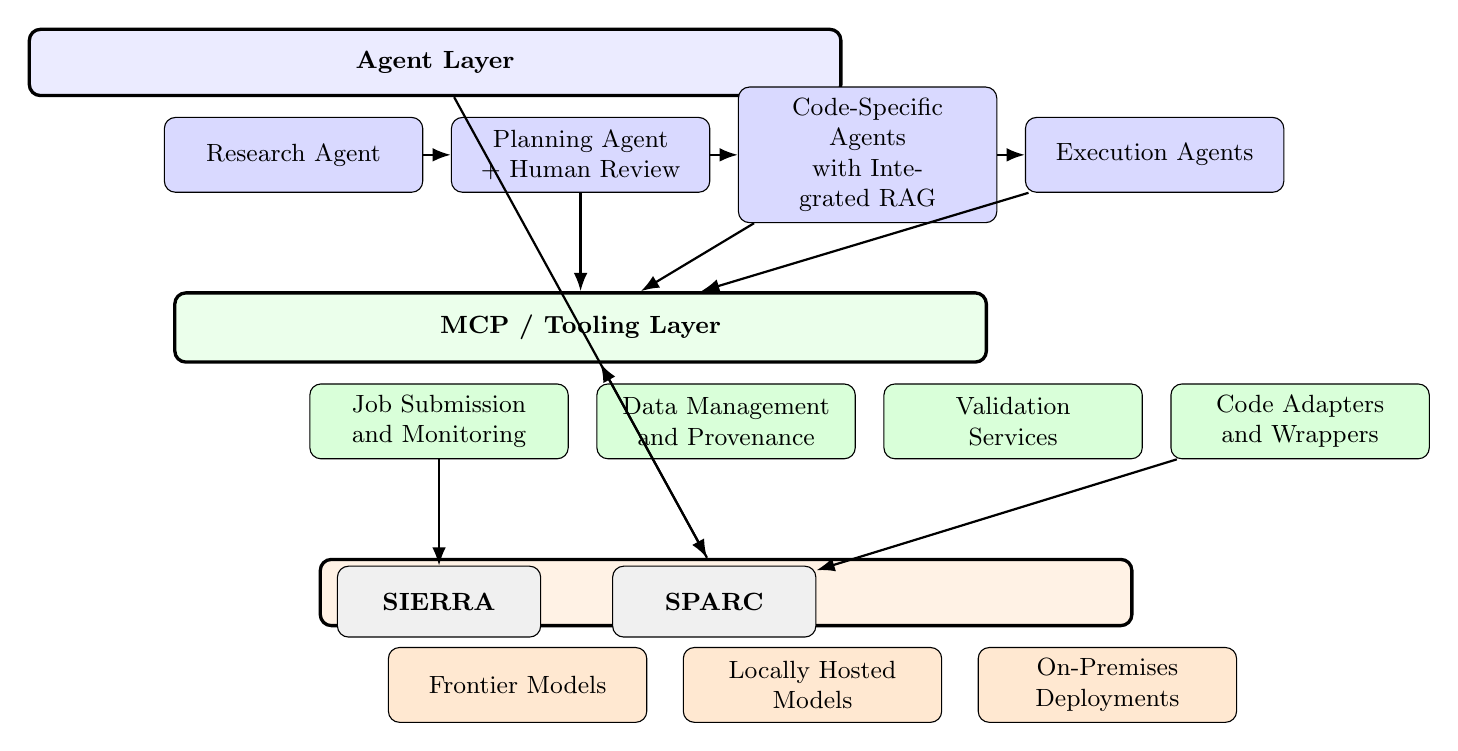
\begin{tikzpicture}[
  font=\small,
  >=Latex,
  node distance=0.45cm and 0.55cm,
  layer/.style={draw, rounded corners, very thick, minimum width=0.85\textwidth, align=center, inner sep=8pt},
  box/.style={draw, rounded corners, align=center, minimum height=0.95cm, text width=3.0cm, inner sep=4pt},
  codebox/.style={draw, rounded corners, align=center, minimum height=0.9cm, text width=2.3cm, inner sep=4pt},
  flow/.style={->, thick}
]
\node[layer, fill=blue!8] (agent) {\textbf{Agent Layer}};
\node[box, fill=blue!15, below left=0.25cm and 0.15cm of agent.south] (research) {Research Agent};
\node[box, fill=blue!15, right=0.35cm of research] (planner) {Planning Agent\\+ Human Review};
\node[box, fill=blue!15, right=0.35cm of planner] (codeagents) {Code-Specific Agents\\with Integrated RAG};
\node[box, fill=blue!15, right=0.35cm of codeagents] (exec) {Execution Agents};

\node[layer, fill=green!8, below=1.25cm of planner] (mcp) {\textbf{MCP / Tooling Layer}};
\node[box, fill=green!15, below left=0.25cm and 0.15cm of mcp.south] (jobs) {Job Submission\\and Monitoring};
\node[box, fill=green!15, right=0.35cm of jobs] (data) {Data Management\\and Provenance};
\node[box, fill=green!15, right=0.35cm of data] (validate) {Validation\\Services};
\node[box, fill=green!15, right=0.35cm of validate] (adapters) {Code Adapters\\and Wrappers};

\node[layer, fill=orange!10, below=1.25cm of data] (llm) {\textbf{LLM Layer}};
\node[box, fill=orange!18, below left=0.25cm and 1.0cm of llm.south] (frontier) {Frontier Models};
\node[box, fill=orange!18, right=0.45cm of frontier] (local) {Locally Hosted\\Models};
\node[box, fill=orange!18, right=0.45cm of local] (prem) {On-Premises\\Deployments};

\node[codebox, fill=gray!12, below=1.35cm of jobs] (sierra) {\textbf{SIERRA}};
\node[codebox, fill=gray!12, right=0.9cm of sierra] (sparc) {\textbf{SPARC}};

\draw[flow] (research) -- (planner);
\draw[flow] (planner) -- (codeagents);
\draw[flow] (codeagents) -- (exec);
\draw[flow] (planner) -- (mcp);
\draw[flow] (codeagents) -- (mcp);
\draw[flow] (exec) -- (mcp);
\draw[flow] (agent) -- (llm);
\draw[flow] (jobs) -- (sierra);
\draw[flow] (adapters) -- (sparc);
\draw[flow] (llm) -- (mcp);
\end{tikzpicture}
\caption{Proposed GENESIS-AGENT architecture. Retrieval is integrated into the
code-specific agents, MCP services mediate workflow execution, and the backend
LLM interface remains deployment-agnostic.}
\label{fig:genesis-architecture}
\end{figure}
\end{comment}
%\subsection*{Technical Approach}
Our proposed work in Phase I can be classified by three aims: (i) the development of structured representations of scientific workflows and modeling and simulation that agents can reason over, (ii) the development of task-specific agents and MCP severs to enable plug-and-play integration with different agentic techologies, and (iii) end-to-end demonstration and evaluation. These aims are now described. 
%Methodologically, the Phase I effort will focus on several open questions that
%we view as central to this area. First, how should simulation workflows be
%represented so that agents can reason over them reliably and in a verifiable
%way? Second, how should retrieval be integrated into code-specific reasoning
%for DOE software, much of which is proprietary and absent from LLM training
%data? Third, what is the right level of abstraction for MCP interfaces so that
%they are reusable without becoming brittle? Finally, how should validation and
%human review be coupled to agent decisions so that the resulting system is
%trustworthy and auditable?
%\bertmargin{Will the end-user create these graphs, or will we build an agent that will generate these graphs for review by a human before starting to run them.}
\paragraph{Aim 1: Structured workflow representations for agentic scientific computing.} A central technical challenge in GENESIS-AGENT is to define structured workflow representations for scientific reasoning that agents can reliably reason over, verify, and refine under human supervision. 
Inspired by the NexGen workflow system within Sandia's Analysis Workbench, we propose representing these workflows with a structured graph, whose nodes represent tasks (e.g., input generation, execution, analysis), and whose edges encode data dependencies and outputs. In Phase I, we will develop schema-based representations for a myriad of such reasoning graphs, and develop agents that can reason over these graphs, propose new graphs from novel user prompts, and refine the graph with human interaction. Here we will 
focus on decomposing outer-loop analyses into executable tasks, required inputs and files, validation checks, model execution, and outputs. These representations serve as the glue between user requests, agent reasoning, simulation codes, and outer-loop analysis tools, and root planning and execution in explicit workflow objects that can be inspected by users, validated automatically, and reused across codes and workflows.
\textit{Lead:
[PI/Co-PI names]. Budget: [insert amount or \% effort].}
%\wyattmargin{I think the use of MCP here is critical and a solid choice. I wanted to mention, however, that we might want to also use agent skills in other places as they tend to be more lightweight to use and easy to work with, though with added risk.}

\paragraph{Aim 2: Specialized agent development and orchestration with MCP-enabled tool use.}
Building on the workflow representations from Aim 1, we will develop a hierarchical suite of task-specific agents that plan, execute, and refine scientific workflows, along with an orchestration framework to interweave these agents into end-to-end reasoning. To enable scalability across diverse environments, we represent task-specific capabilities as tools and constrain the tools available to each agent, exposing only what is necessary to support reasoning and mitigate drift from intended use.
While the long-term (Phase II) vision includes a \textit{research agent} capable of synthesizing diverse data sources to formulate new hypotheses, Phase I will focus on a \textit{reasoning agent} that iterates on and decomposes a well-defined hypothesis into a structured workflow and coordinates downstream actions. This process is explicitly \textit{human-in-the-loop}: the agent proposes a workflow, presents it for review, and refines it based on feedback prior to execution. Once finalized, the planner interfaces with \emph{specialized agents}, including code-specific agents for simulation tools and \textit{execution agents} for HPC job submission and management. Code-specific agents encode knowledge of input-deck construction, solver configuration, execution workflows, and post-processing, while execution agents encode knowledge of HPC environments and resource constraints.

To enable these agents to operate across DOE’s complex ecosystem, we will develop retrieval-augmented generation (RAG) pipelines that synthesize relevant context into the decision process. These pipelines treat documentation, prior workflows, and validated inputs as retrievable knowledge sources, enabling deployment on codebases not present in LLM training. To manage multimodal information, retrieval will leverage hybrid search strategies~\cite{edge2025localglobalgraphrag,formal2021spladesparselexicalexpansion,yue2026foamagentautomatedintelligentcfd}, combining embedding-based similarity searches with keyword matching and metadata constraints.

To support reusable, secure, and standardized access to tools, we will integrate the Model Context Protocol (MCP) as the primary interface layer for shared capabilities. In this architecture, agents reason over structured workflow objects and invoke MCP services when interacting with external systems or reusable components, creating a clean separation between reasoning and execution. This abstraction also insulates GENESIS-AGENT from the rapidly evolving agentic AI landscape. By exposing capabilities through MCP, they remain accessible to any compatible framework, enabling interoperability with both internally developed and commercial systems. For example, an agent specialized in constructing simulation input decks can expose its functionality as a callable tool, allowing external frameworks (e.g., Claude or Codex) to leverage DOE-specific expertise while preserving control over interfaces, execution, and security.
At the same time, we recognize a complementary design space in which lighter-weight \emph{agent skills} may be used for tightly scoped or highly specific tasks, trading stronger standardization and control for increased flexibility and ease of development. We will explicitly study this tradeoff, using MCP for stable, reusable, capabilities, while leveraging agent skills where lightweight integration is advantageous.



\begin{comment}
\paragraph{Aim 2: Specialized agent development and orchestration with MCP-enabled tool use.} Building on the workflow representations from Aim 1, we will develop a hierarchical suite of task-specific agents that plan, execute, and refine scientific workflows, along with the development of the orchestration framework to interweave these agents to achieve end-to-end reasoning. In defining this hierarchy, we address the ability of agentic workflows to scale to diverse environments by representing task-specific agents as tools, and subsequently constraining the tools available to each agent, exposing only what is necessary to facilitate agent reasoning and mitigate agents that drift from their intended use. 

While we ultimately envision a \textit{research agent} capable of parsing diverse data sources to formulate new hypotheses, in Phase I we will start with a \textit{planning agent} that decomposes a pre-defined hypothesis or user request into a structured workflow and coordinates downstream actions. The planning agent will be explicitly centered on \textit{human-in-the-loop} interactions: leveraging the structured workflow representations defined in Aim 1, the agent will propose an initial plan, present the resulting workflow representation for human review, and revise that plan based on feedback before execution proceeds. Once finalized, the planner will interface with a collection of \emph{specialized agents}, including code-specific agents tailored to individual simulation tools (e.g., Sierra/Aria, OpenFOAM, Dakota) and \textit{execution agents} tailored to submitting and managing HPC jobs. The code-specific agents will encode detailed knowledge of input-deck construction, solver configuration, execution workflows, and post-processing, while the execution agents will encode knowledge of HPC environments, resource availability, and job submission. To facilitate the ability of these agents to navigate DOE's complex computational ecosystem, we will develop retrieval augmented generation (RAG) pipelines to synthesize relevant context into the decision process. These tool-specific retrieval pipelines will treat documentation, prior workflows, and validated inputs as retrievable knowledge sources at inference time, thereby enabling deployment on codebases not seen within LLM training. To effectively manage multimodal information, these retrieval pipelines will leverage hybrid search strategies~\cite{edge2025localglobalgraphrag,formal2021spladesparselexicalexpansion,yue2026foamagentautomatedintelligentcfd}, combining, for example, similarity searches on embeddings with keyword matching and metadata
constraints to identify relevant context. 


To support reusable and standardized access to tools, we
will integrate the Model Context Protocol (MCP) as the interface layer for
shared capabilities. 
In this architecture, agents reason over structured workflow objects and invoke
MCP services when interaction with specialized agents or reusable software
components is required, creating a clean separation between reasoning and
execution. This abstraction also provides insulation from the rapidly evolving
landscape of agentic AI. Rather than coupling GENESIS-AGENT to a specific
framework, MCP enables interoperability with both internally developed and
commercial agentic systems.
By defining capabilities through MCP, they
can be accessed by any agentic framework that supports the protocol. For
example, an agent specialized in constructing input decks for a physics
simulation can expose its functionality as a callable tool, enabling external
frameworks (e.g., Claude or Codex) to leverage DOE-specific expertise while preserving
control over interfaces, execution, and security.

%A central research question in this aim is the choice of interface granularity: MCP interfaces that are too fine-grained become delicate and increase the probability of inappropriate tool use, while interfaces that are too coarse reduce reuse across workflows. In parallel, we will develop retrieval-augmented generation (RAG) pipelines so that code-specific agents can ground their decisions in technical documentation, prior workflows, and validated inputs that are not present in model training data. These retrieval pipelines will leverage hybrid search strategies~\cite{edge2025localglobalgraphrag,formal2021spladesparselexicalexpansion,yue2026foamagentautomatedintelligentcfd}, combining similarity search over embeddings with keyword matching and metadata constraints to identify relevant context at inference time.  \textit{Lead: [PI/Co-PI names].  Budget: [insert
%amount or \% effort].}
%}
\end{comment}
\begin{comment}
\textbf{Aim 1: Structured agent orchestration and workflow representations.}
The primary research contribution of this project is the development of a structured framework for coordinating role-specialized agents across the modeling and simulation lifecycle. Rather than treating agent interactions as loosely coupled prompt exchanges, we will develop workflow representations that explicitly encode task decomposition and task dependencies. These representations will serve as the layer over which agents reason, communicate, and compose multi-stage workflows.

We will design a hierarchical orchestration framework in which a planning agent maps high-level scientific intent to a structured workflow graph, whose nodes represent tasks (e.g., input generation, execution, analysis) and whose edges encode data and control dependencies. Downstream agents—including code-specific agents for simulation tools (e.g., SIERRA, OpenFOAM), execution agents for HPC environments, and analysis agents for post-processing—will operate over this shared representation, ensuring consistency across stages and enabling partial execution, validation, and refinement.

A key component of this aim is the integration of hybrid retrieval into the workflow representation. Rather than retrieving unstructured documents alone, we will develop retrieval pipelines that surface structured artifacts—such as prior workflows, validated input configurations, and execution traces—and align them with the workflow graph. This enables agents to ground their decisions in both semantic context and executable precedent, improving robustness in settings where training data is incomplete or unavailable.

Finally, we will investigate mechanisms for verification and correction within this structured setting. By operating over explicit representations of dependencies and artifacts, the system can detect inconsistencies (e.g., mismatched boundary conditions, invalid parameter couplings), localize errors to specific workflow components, and trigger targeted refinement cycles. This transforms agentic reasoning from a purely generative process into a constrained, verifiable computation over structured scientific workflows.


\paragraph{Aim 1: Specialized agent development and orchestration.} At the core of GENESIS-AGENT is our proposed approach to address the development of an agnetic system that can scale to the myriad of tools in use at DOE. Specifically, we propose the development of a hierarchical suite of task-specific agents responsible for different
aspects of the scientific process, and the development of the orchastration framework to interweave these agents to achieve end-to-end workflows. In defining this hierarchy, we will constrain the tools available to each agent, exposing only what is necessary to facilitate agent reasoning and mitigate agents that drift from their intended use. 

We ultimately envision \textit{research agents} capable of parsing multimodal data sources to develop
novel research hypotheses and tasks. In Phase I, however, we propose starting at the development of \textit{planning agents} that can refine a well-defined hypothesis or
request and synthesize it into a series of tasks and coordinate downstream results to recommend further action. The planning agent will be explicitly centered on \textit{human-in-the-loop} interactions: it will generate an initial plan, present that plan to a human reviewer, and
then iterate based on feedback. Once finalized, the planner will interface with a collection of \emph{specialized agents}, including code-specific agents tailored to individual simulation tools (e.g., Sandia's Sierra codebase) and \textit{execution agents} tailored to submitting and managing HPC jobs. The code-specific agents will encode detailed knowledge of input-deck
construction, solver configurations, execution workflows,
and post-processing, while the execution agents will encode knowledge of HPC environments, resource availability, and job submission. These agents will be constructed through feature engineering and task-specific
design.

Retrieval is additionally a central component of this aim. To facilitate the ability of these agents to navigate DOE's complex computational ecosystem, we will develop retrieval augmented generation (RAG) pipelines to synthesize relevant context into the decision process. These tool-specific retrieval pipelines will treat documentation, prior workflows, and validated inputs as retrievable knowledge sources at inference time, thereby enabling deployment on codebases not seen within LLM training. To effectively manage multimodal information, these retrieval pipelines will leverage hybrid search strategies~\cite{edge2025localglobalgraphrag,formal2021spladesparselexicalexpansion,yue2026foamagentautomatedintelligentcfd}, combining, for example, similarity searches on embeddings with keyword matching and metadata
constraints to identify relevant context. \textit{Lead:
[PI/Co-PI names]. Budget: [insert amount or \% effort].}


\paragraph{Aim 2: MCP tooling.} A myriad of actions required to complete end-to-end analyses, such as job submisison, minitoring, and post processing, are reusable and can be shared across different agents. Constructing infrastructure to faciliate this reuse is key to scalability. Further more, the landscape in agentic AI is rapidly evolving, and it is within reason to expect that commercially developed agentic frameworks will outpace those that which can be developed within DOE. To enable scalability and facilitate integration into heterogeneous agentic tools, we will build MCP severs for a myriad of task-specialized agents. Critically, the construction of these MCP servers enables task-specialized agentic technologies to be exposed to any agentic framework that supports MCP. In this setting, an agent specialized for, e.g., constructing an input deck for a physics simulation can directly provide a toolset for a commercial agentic AI system, such as Codex.
%While the main focus will be integration of these tools into GENESIS-AGENT, we propose to develop them in a stand-alone manner such they can be broadly accessed and provide MCP tools of general use to DOE. We emphasize that, while various MCP tools are stand-alone actions, more sophisticated ones may be agentic systems themselves. 
A central research question we aim to address is the choice of interface granularity: interfaces that are too fine-grained become delicate and increase the probability of inappropriate tool use, while interfaces that are too coarse reduce reuse across codes.  \textit{Lead: [PI/Co-PI names].  Budget: [insert
amount or \% effort].}
\end{comment}
\paragraph{Aim 3: End-to-end demonstration of closed-loop scientific reasoning.} The third aim is to integrate the full pipeline into an end-to-end demonstrate in which the system synthesizes a natural language hypothesis, proposes a structured plan for an outer-loop
analysis, refines the plan with a human reviewer, generates the necessary simulation and analysis inputs, executes
the workflow, interprets the outputs, and returns recommended follow-on actions. The demonstration will demonstrate that GENESIS-AGENT can recommend actions and complete analyses across at least two outer-loop analysis drivers, including Dakota, and at least three physics codebases: SIERRA/Solid Mechanics, SPARC, and OpenFOAM. \textit{Lead: [PI/Co-PI names]. Budget:
[insert amount or \% effort].}

\section{Milestones in the Nine Months}
The Phase I effort is organized around five milestones that move from fine-grained, code specialized agents to multi-agent frameworks and demonstrations. We structure the objectives in this way as they represent a risk-hierachy and maximize potential impact: specialized agents for physics codes can still provide an AI advantage even if full end-to-end demonstrations prove untenable. 

\begin{itemize}[leftmargin=1.2em,itemsep=0.2em,topsep=0.2em]
\item \textbf{Milestone 1: Specialized agents for physics codes (Months 1--3).}
Develop agents specialized to candidate physics codebases, including
SIERRA/Solid Mechanics, SPARC, and the OpenFOAM thread that builds from
FOAM-agent. These agents will encode knowledge of relevant physics, schemas,
and execution commands, and they will support input generation, consistency
checks, and error detection for candidate simulation workflows.
\textit{Completion criterion: code-specific agents generate candidate inputs
and pass basic validation checks for the selected benchmark problems.}

\item \textbf{Milestone 2: Specialized agents for outer-loop analyses (Months
2--4).} Develop agents specialized to the setup and execution of outer-loop
analyses using Dakota or a related tool (PyTUQ, rom-tools-and-workflows). These agents
will translate natural-language requests into structured study definitions,
formulate execution plans, and orchestrate downstream analysis tasks through
validated workflow objects. \textit{Completion criterion: at least one
outer-loop agent produces valid study definitions and executable plans for
representative benchmark problems.}

%\item \textbf{Milestone 3: Agent orchestration and workflow representations
%(Months 1--5).} Define the core architecture for GENESIS-AGENT, including
%workflow schemas, the initial data and document sources used for retrieval,
%provenance structures, and benchmark problems. This milestone will establish
%the structured representations needed to connect outer-loop analyses,
%physics-code workflows, and human review within a common framework.
%\textit{Completion criterion: a documented architecture, an initial benchmark
%suite, and working schema definitions for both outer-loop and physics-code
%workflows.}

\item \textbf{Milestone 3: Agent orchestration and workflow representations
(Months 1--5).} Establish the core architectural contribution of
GENESIS-AGENT: a structured framework for coordinating role-specialized agents
across the modeling and simulation lifecycle. We will develop workflow schemas
that formalize how agents decompose tasks, exchange context, and compose
multi-stage workflows. \textit{Completion criterion: a documented architecture, an initial
benchmark suite, and validated schema definitions enabling coordinated,
multi-agent execution across coupled workflows.}


\item \textbf{Milestone 4: MCP integration, validation, and secure execution
(Months 4--7).} Implement MCP services for reusable actions such as job
submission, monitoring, data management, validation, and provenance capture.
This milestone will also study the appropriate abstraction level for MCP
interfaces so that they remain reusable across tools while still supporting
reliable and auditable execution in DOE environments. \textit{Completion
criterion: representative MCP services operate through a common interface and
support auditable execution for the selected workflows.}

\item \textbf{Milestone 5: End-to-end demonstration and evaluation (Months
7--9).} Integrate the full pipeline and demonstrate an end-to-end
human-in-the-loop workflow spanning outer-loop analysis planning, input
generation, simulation execution, and post-processing. This milestone will
include demonstration with multiple analysis drivers and multiple physics
codes, including SIERRA and SPARC, and will provide the main evidence for AI
advantage at the end of Phase I. \textit{Completion criterion: successful
execution of the end-to-end workflow for the selected demonstration cases and
evaluation against the Phase I decision metrics.}
\end{itemize}

\begin{comment}
\begin{figure}[t]
\centering
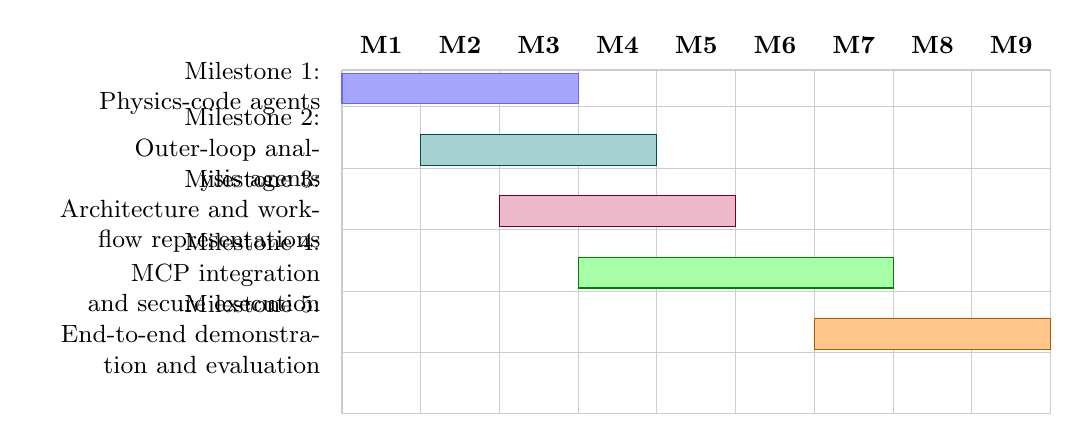
\begin{tikzpicture}[x=1.0cm,y=0.78cm,font=\small]
\foreach \x/\m in {1/1,2/2,3/3,4/4,5/5,6/6,7/7,8/8,9/9} {
  \node at (\x,6.2) {\textbf{M\m}};
  \draw[gray!40] (\x-0.5,0.2) -- (\x-0.5,5.8);
}
\draw[gray!40] (9.5,0.2) -- (9.5,5.8);
\foreach \y in {0.2,1.2,2.2,3.2,4.2,5.2,5.8} {
  \draw[gray!40] (0.5,\y) -- (9.5,\y);
}
\node[anchor=east,align=right,text width=3.6cm] at (0.35,5.5) {Milestone 1:\\Physics-code agents};
\node[anchor=east,align=right,text width=3.6cm] at (0.35,4.5) {Milestone 2:\\Outer-loop analysis agents};
\node[anchor=east,align=right,text width=3.6cm] at (0.35,3.5) {Milestone 3:\\Architecture and workflow representations};
\node[anchor=east,align=right,text width=3.6cm] at (0.35,2.5) {Milestone 4:\\MCP integration and secure execution};
\node[anchor=east,align=right,text width=3.6cm] at (0.35,1.5) {Milestone 5:\\End-to-end demonstration and evaluation};

\filldraw[fill=blue!35,draw=blue!60] (0.5,5.25) rectangle (3.5,5.75);
\filldraw[fill=teal!35,draw=teal!60!black] (1.5,4.25) rectangle (4.5,4.75);
\filldraw[fill=purple!28,draw=purple!60!black] (2.5,3.25) rectangle (5.5,3.75);
\filldraw[fill=green!35,draw=green!50!black] (3.5,2.25) rectangle (7.5,2.75);
\filldraw[fill=orange!45,draw=orange!70!black] (6.5,1.25) rectangle (9.5,1.75);
\end{tikzpicture}
\caption{Nine-month Gantt chart for the major Phase I milestones.}
\label{fig:gantt}
\end{figure}
\end{comment}

\section{Data Sources and Models}
The project will not require training or fine-tuning of LLMs, and data-sources will primarily be utilized for retrieval and validation pipelines. For this purpose, we will leverage diverse data sources associated with computational
science workflows, including input decks, documentation, and case
results for the target analysis tools and simulation codes. These materials
will provide the basis for RAG pipelines, feature engineering, and validation. The team already has access to a substantial amount of these data through past work, internal technical materials, and open-source code bases. These sources include the types of technical artifacts already used in prior team efforts such as Foam-Agent. The team is capable of collecting additional supporting data as needed. 

On the model side, the project will intentionally utilize generic APIs so that the framework can integrate with a suite of LLMs rather than depending on a single model
provider. In particular, the effort will focus jointly on frontier models and open-source models currently hosted on premises at Sandia through Shirty Microservices. This will allow us to evaluate both capability and deployment tradeoffs while maintaining a backend-agnostic software architecture. We will also assess integration with and
comparison to existing open-source and commercial agentic frameworks in order to position GENESIS-AGENT relative to the current state of practice.

\section{Decision Gate Metrics}
\bert{If I can be super-critical here: it feels to me that only decision gate 2 qualifies as AI advantage, in the sense that it quantifies the improvement over a manual baseline.
The other two decision gates feel more like ensuring the approach is well-formulated.
Would it make sense to rework this section as ensuring the approach is well posed and once it is well-posed, achieving AI advantage in the form of human effort reduction?
I do love decision gate 3 as it beautifully sets the stage for Phase II.}

\bert{Another thing to keep in mind is that we need to show AI advantage at the 6-month mark.
If end-to-end demonstration does not happen till Months 7 - 9, then we can't have an AI advantage metric that depends on that. 
Can we rework the timetable so that we do the end-to-end demonstration sooner (maybe on a smaller problem set), and then do some generalization, and scaling tests in the last 3 months?}

\wyatt{I will echo a little of what BJD suggested here. I think it is a good idea to have a smaller scale problem we can show end-to-end more quickly. Maybe a workflow for just one of our solvers on a small number of problems? }

Phase I go/no-go decision will be based on whether GENESIS-AGENT
demonstrates a measurable AI advantage on representative benchmark workflows.
%To ensure early validation of this capability, we will perform a reduced-scope
%end-to-end demonstration by Month 6 on a focused set of problems (e.g., a single
%solver and limited benchmark cases), followed by broader generalization and
%scaling studies in Months 7--9. 
Performance will be assessed through three
decision gates:

\begin{itemize}[leftmargin=1.2em,itemsep=0.2em,topsep=0.2em]

\item \textbf{Decision Gate 1: Validation of study generation and execution.}
The system must generate valid studies and successfully execute
representative tasks. By Month 5, a reduced-scope demonstration will show 
end-to-end execution for a study with at least one solver and a limited set of supported analyses. %By the end of Phase I, a successful outcome is that at least 70\% of
%benchmark cases produce valid inputs and at least 50\% complete end-to-end
%execution with bounded human intervention.

\item \textbf{Decision Gate 2: AI advantage through human-effort reduction.}
The system must reduce the expert effort required to set up, validate, and run
representative studies. Initial evidence of AI advantage will be demonstrated
at Month 6 on benchmakrk studies through measurable reductions in
hands-on setup and debugging time relative to a baseline manual study. By
the end of Phase I, the target is at least a $2\times$ reduction on the full
demonstration cases.

\item \textbf{Decision Gate 3: Scaling and adaptation.}
Following the initial demonstration, the system must show improved performance
as additional AI-relevant resources are applied, including expanded retrieval
data, stronger models, or increased tool context. A successful outcome is
monotonic improvement in at least one key metric---such as input validity,
execution success rate, or reduction in human editing burden---as these
resources are increased during Months 7--9.

\end{itemize}

Together, these decision gates ensure that Phase I establishes an early
demonstration of AI advantage on a tractable problem, followed by evidence of
generalization and scalability across more complex workflows. This progression
provides a credible foundation for transformative AI-enabled science and
engineering in Phase II.





\begin{comment}

The Phase I go/no-go decision will be based on whether GENESIS-AGENT
demonstrates a measurable AI advantage on representative benchmark workflows.
This will be assessed through three decision gates:

\begin{itemize}[leftmargin=1.2em,itemsep=0.2em,topsep=0.2em]
\item \textbf{Decision Gate 1: Workflow generation and execution.} The system
must generate valid workflows and successfully execute representative
tasks across the selected benchmark problems. A successful outcome is that at
least 70\% of benchmark cases produce valid inputs and at least 50\% complete
end-to-end execution with bounded human intervention.

\item \textbf{Decision Gate 2: Human-effort reduction.} The system must reduce
the expert effort required to set up, validate, and run representative studies.
A successful outcome is a measurable reduction in hands-on setup and debugging
time relative to a baseline manual workflow, with a target reduction of at
least 2$\times$ on the selected demonstration cases.

\item \textbf{Decision Gate 3: AI advantage through scaling and adaptation.}
The system must show improved performance as additional AI-relevant resources
are applied, including more retrieval data, stronger models, or expanded tool
context. A successful outcome is monotonic improvement in at least one key
metric, such as input validity, execution success rate, or reduction in human
editing burden, when these resources are increased. 
\end{itemize}

Together, these decision gates evaluate whether the Phase I effort has produced
a credible foundation for transformative AI-enabled science and engineering:
the system must work on realistic workflows, reduce expert effort in a
quantifiable way, and exhibit scaling behavior that supports continued
improvement in Phase II.
\end{comment}
\clearpage \appendix \section*{Appendix 1: Bibliography and References Cited}
\nocite{dakota_docs}
\nocite{romtools_workflows}
\bibliographystyle{plain}
\bibliography{refs}

\end{document}
